\section{Proposed Work} % or "Research Plan"
\label{sec:proposed}

Describe your proposed work here. You may refer to other sections so as not to
repeat yourself -- for example, referencing Section~\ref{sec:background}.

You may want to use figures to illustrate your point, such as
Figure~\ref{fig:sample}.

\begin{figure}[h]
 \centering % avoid the use of \begin{center}...\end{center} and use \centering instead (more compact)
 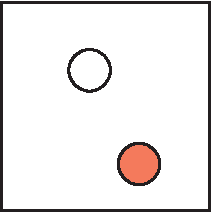
\includegraphics[width=1.5in]{figs/sample}
 \caption{Figure illustrating some proposed desgins.}
 \label{fig:sample}
\end{figure}

\subsection{Data}
\label{sec:data}

Describe the data and your access to it here.

\subsection{Evaluation}
\label{sec:eval}

Describe your plan for evaluating your work, even if it does not fit in the
timeframe of this project. Without time constraints, what would you? Do you
have the resources (people, time, equipment, data, money) to implement this
plan in the future?

\subsection{Timeline}
\label{sec:timeline}

Set up milestones for your project and  summarize in Table~\ref{tab:milestones}.

\begin{table}[h]
%% Table captions on top in journal version
 \caption{Project Milestones}\vspace{1ex} % the \vspace adds some space after the top caption
 \label{tab:milestones}
 \scriptsize
 \centering % avoid the use of \begin{center}...\end{center} and use \centering instead (more compact)
   \begin{tabular}{r|r}
     Date & Milestone (\%)\\
   \hline
     Sep 30 & Interviews conducted, initial task abstractions\\
     Oct  2 & Five datasets uploaded \\
     Oct  7 & Initial design sketches\\
     Oct 14 & Paper prototypes of 3 initial designs\\
     Oct 21 & Wireframe of central design \\
     Nov 7 & Initial prototype of design 
   \end{tabular}
\end{table}

